


\section{Auswertung}
\label{sec:auswertung}

In diesem Kapitel werden die aufgenommenen Messwerte ausgewertet.
\subsection{Der Invertierende-Linearverstärker}
\label{sec:linearverstaerker}
Bei dieser ersten Schaltung wurden für zwei verschiedene Widerstandsverhältnisse Eingangs- und Ausgangsspannung,
$U_a$ und $U_e$, sowie der zeitliche Versatz $\Delta t$ der beiden Signalamplituden vom Oszilloskop abgelesen. 
Zunächst wird dann der Verstärkungsfaktor $x$ mithilfe der von \autoref{eq:vfaktor} berechnet und in 
\autoref{fig:linearverstaerker} gegen die Frequenz $f$ des Eingangsignals aufgetragen. Der Phasenverschiebungswinkel
$\phi$ wurde dann über \autoref{eq:phasenverschiebung} errechnet und in \autoref{fig:phasenverschiebung} 
ebenfalls gegen die Frequenz aufgetragen.

\begin{equation}
    \label{eq:vfaktor}
    x=\frac{U_a}{U_e}
\end{equation}

\begin{equation}
    \label{eq:phasenverschiebung}
    \phi=2\pi f \Delta t
\end{equation}

\label{sec:linearverstaerker}
\begin{figure}
    \centering
    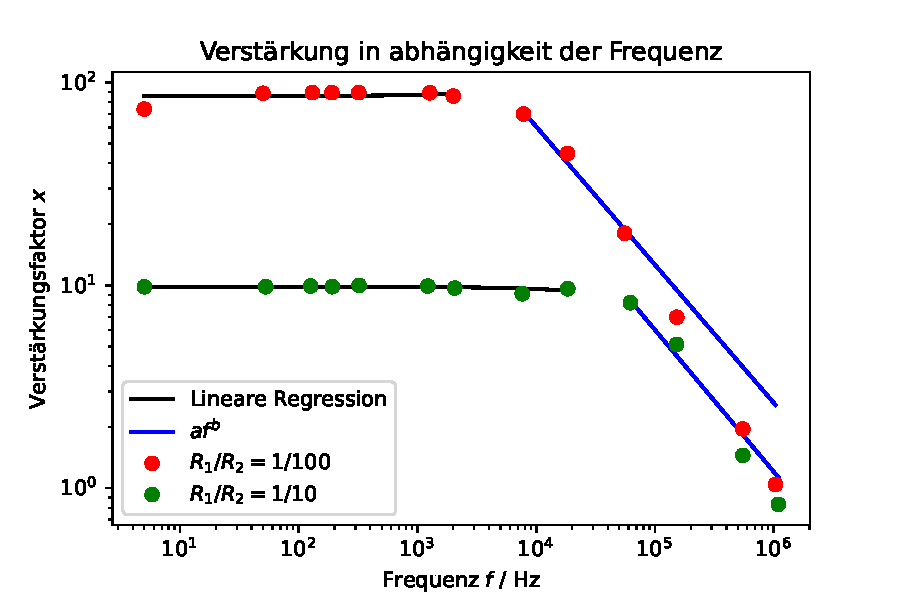
\includegraphics{content/grafiken/verstaerkung.pdf}
    \caption{Verstärkungskurve des als invertierenden Linearverstärker geschalteten Operationsverstärkers nach Eingangsfrequenz.}
    \label{fig:linearverstaerker}
  \end{figure}
  An die konstanten Plateubereiche der Verstärkungskurve wurde je eine Grade nach der Vorschrift $x(f)=af+b$ 
  mit den Parametern:
   \begin{center}
       $a_{1/100} =  0.001\pm 0.003$\\
       $b_{1/100} = 85.819\pm 2.946$\\
       $a_{1/10}  =  0.000\pm 0.000$\\
       $b_{1/10}  = 9.834 \pm 0.095$\\
   \end{center}
 angepasst. Die Steigungen $a_{1/100}$ und $a_{1/10}$ sind vernnachlässigbar klein so das die Verstärkung
 hier als Konstant betrachtet werden kann. An die in der gewählten doppelt-logarithmischen Darstellung
 Funktionsabfälle wurden hingegen Kurven der Vorschrift: 
 \begin{equation}
    \label{eq:exponentialgesetz}
    x=cf^d
 \end{equation}
  angepasst. Daraus folgen die Parameter:
  \begin{center}
    $c = 32076.147  \pm 16619.806$\\
    $d =   -0.681 \pm 0.056$\\
    $c = 18911.087 \pm 21201.677$\\
    $d =   -0.699 \pm 0.099$\\
  \end{center}
  \begin{figure}
    \centering
    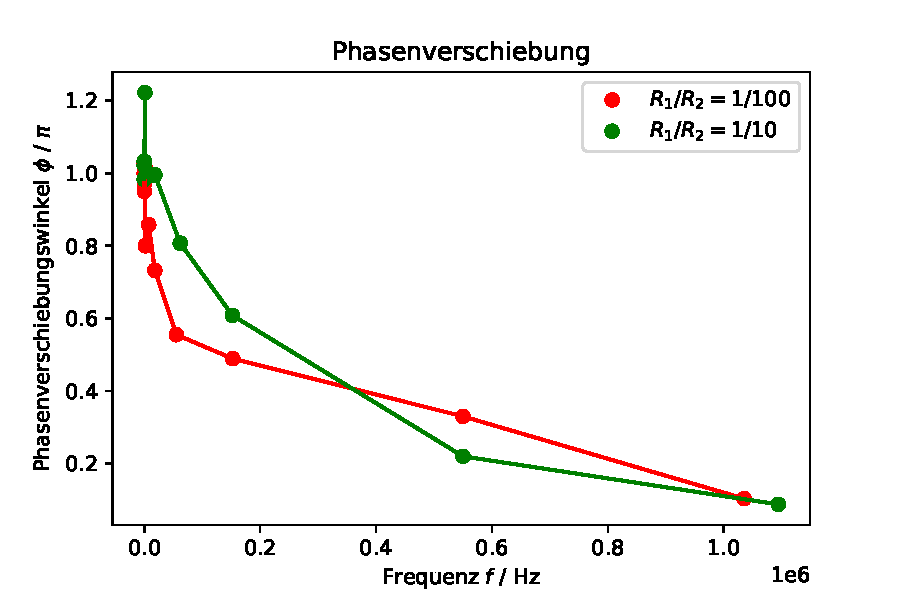
\includegraphics{content/grafiken/phasenverschiebung.pdf}
    \caption{Phasenverschiebung am invertierenden Linearverstärker in Abhängigkeit der Zugangsfrequenz.}
    \label{fig:phasenverschiebung}
  \end{figure}



\subsection{Der Umkehrintegrator und der invertierender Differenzierer}
\label{sec:umkehrintegrator}
\begin{figure}
    \centering
    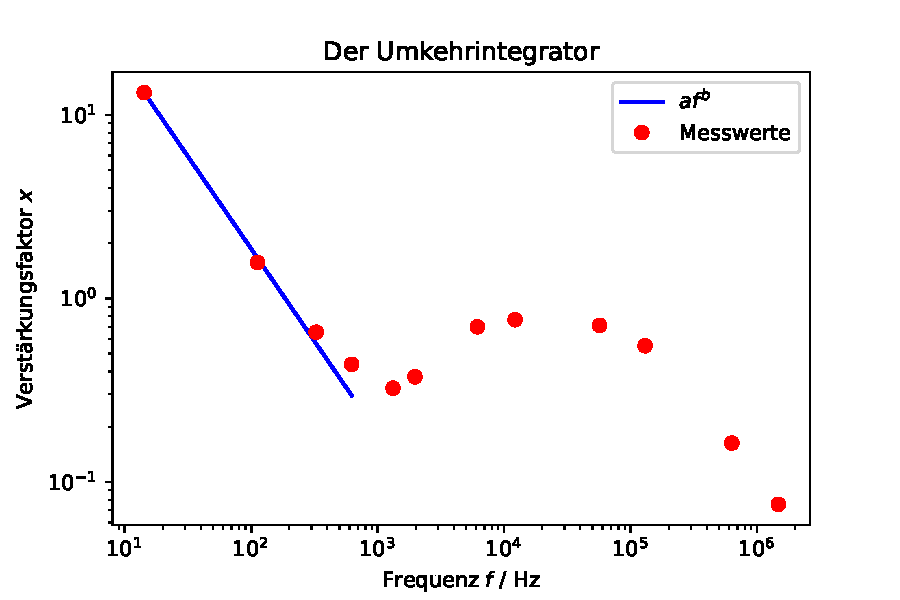
\includegraphics{content/grafiken/umkehrintegrator.pdf}
    \caption{Verstärkungskurve des Umkehrintegrators nach Eingangsfrequenz}
    \label{fig:umkehrintegrator}
  \end{figure}


  \begin{figure}
    \centering
    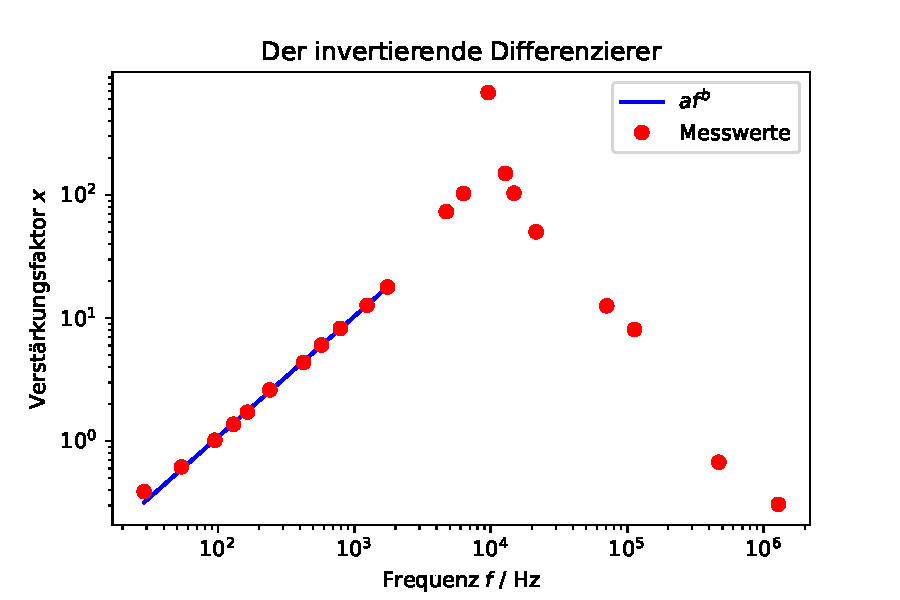
\includegraphics{content/grafiken/invdifferenzierer.pdf}
    \caption{Verstärkungskurve des invertierenden Differenzierers nach Eingangsfrequenz.}
    \label{fig:invdifferenzierer}
  \end{figure}





\subsection{Nicht-invertierender-Schmitt-Trigger}
\label{sec:schmitt}
\begin{figure}
    \centering
    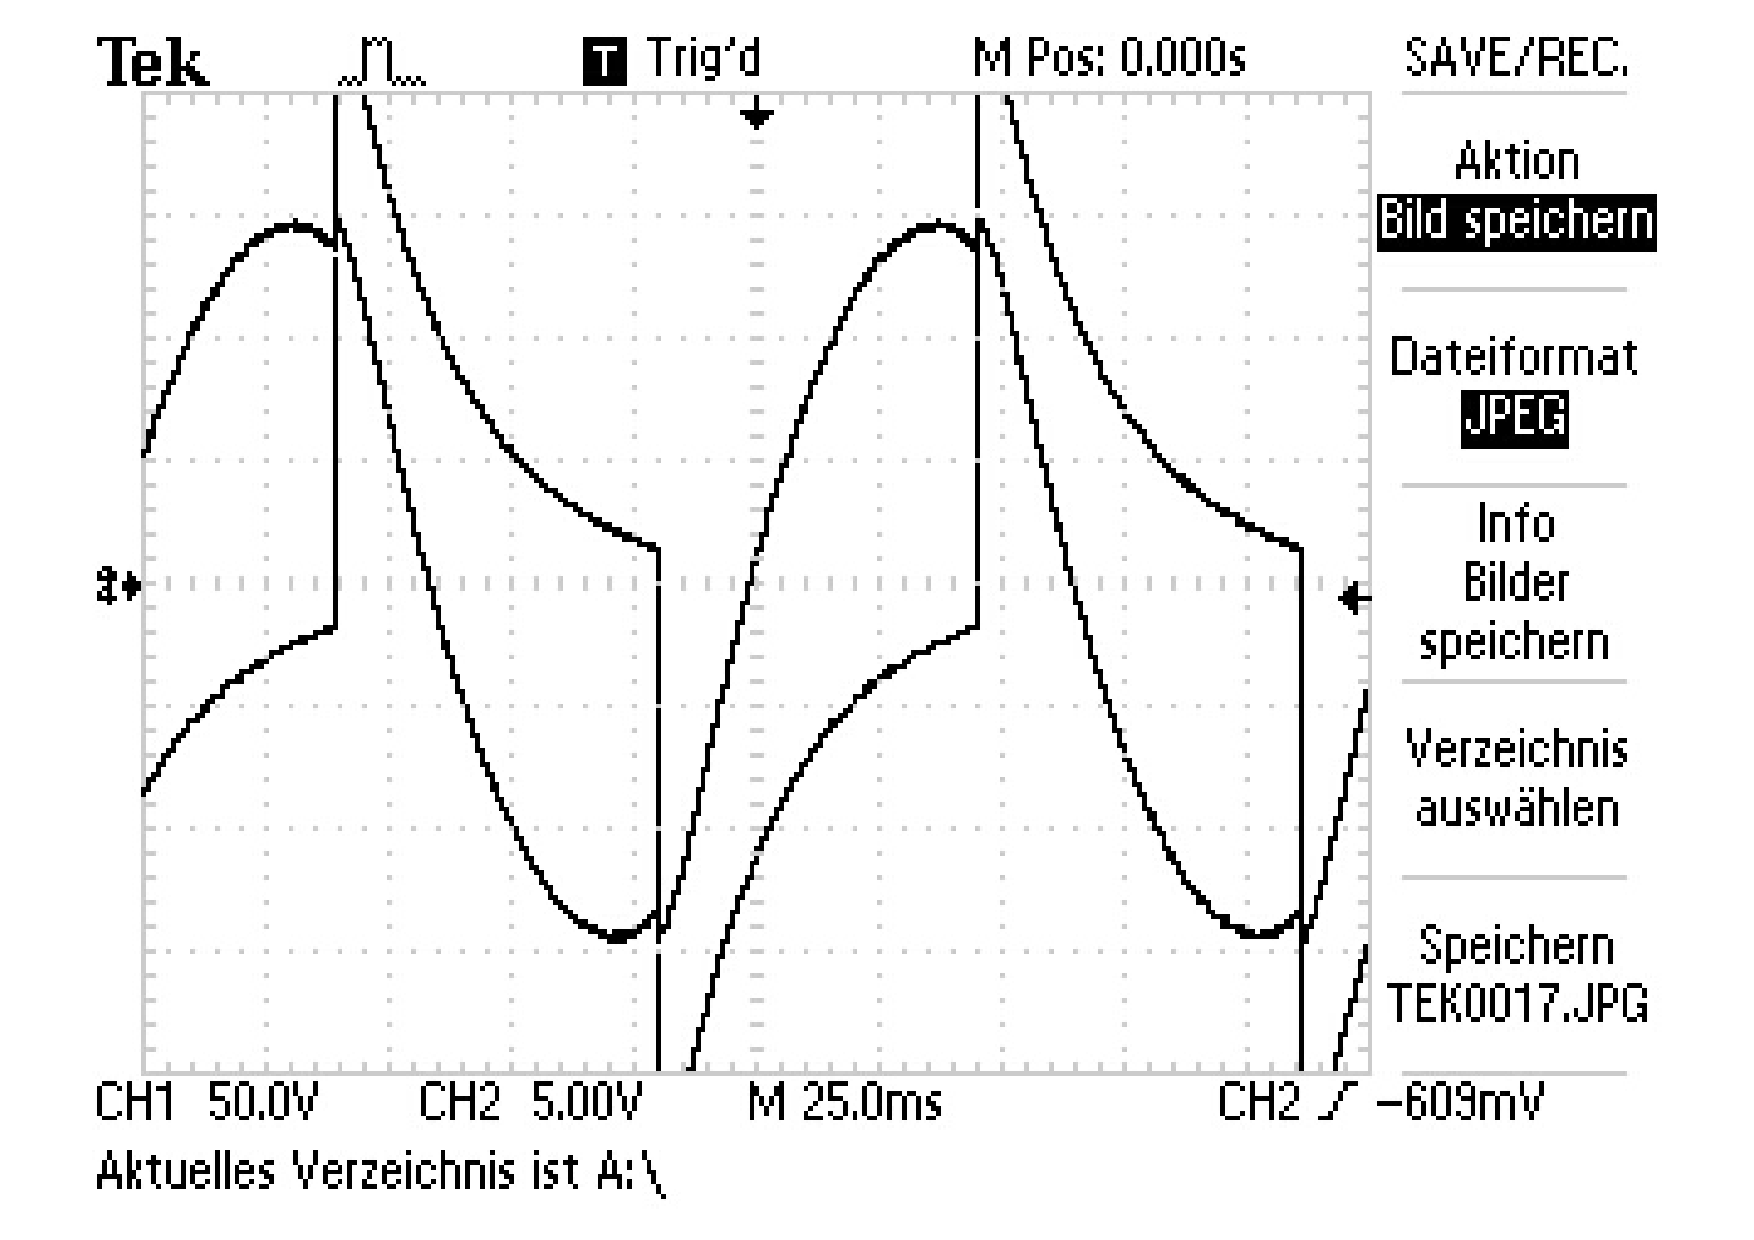
\includegraphics[width=1\textwidth]{content/grafiken/schmittTrigger/TEK0017.pdf}
    \caption{Oszilloskopbild des Spannungsverlaufs am invertierenden Schmitttrigger.}
    \label{fig:schmitttrigger}
  \end{figure}



























